\documentclass[a4paper,10pt]{article}
\usepackage[utf8]{inputenc}
\usepackage{amsmath,amsfonts,amssymb,graphicx,subfigure,mathtools}
\usepackage{amsmath}
\usepackage{rotating}
\usepackage{lscape}
\usepackage{xfrac}

\newcommand{\conj}[1]{\overline{#1}}

%MATRIX HELPER FUNCTIONS
\newcommand\coolover[2]{\mathrlap{\smash{\overbrace{\phantom{%
    \begin{matrix} #2 \end{matrix}}}^{\mbox{$#1$}}}}#2} 

\newcommand\coolunder[2]{\mathrlap{\smash{\underbrace{\phantom{%
    \begin{matrix} #2 \end{matrix}}}_{\mbox{$#1$}}}}#2}

\newcommand\coolleftbrace[2]{%
#1\left\{\vphantom{\begin{matrix} #2 \end{matrix}}\right.}

\newcommand\coolrightbrace[2]{%
\left.\vphantom{\begin{matrix} #1 \end{matrix}}\right\}#2}



%opening
\title{Two dimensional Cavalieri Integral}
\author{T.L. Grobler}

\begin{document}

\maketitle

\begin{section}{Extension}

$\mathcal{C} = \{L,S\}$ and $\Delta x_{ij}^1 = x_{i+1,j}^1 - x_{ij}^1$. $L$ is a parametric curve that intersects region $S$ at $(x_{ij}^1,y_{ij}^1)$ and surface 
$f$ at $(x_{ij}^2,y_{ij}^2)$.


\begin{eqnarray}
\iint\limits_{\!\mathcal{C}} f(x,y) dA &=& \lim_{n,m\rightarrow \infty} \sum_{j=1}^n\sum_{i=1}^n f(x_{ij}^2,y_{ij}^2) \Delta x_{ij}^1\Delta y_{ij}^1\\
&=&  \lim_{n,m\rightarrow \infty} \sum_{j=1}^n\sum_{i=1}^n f(g(x_{ij}^1,y_{ij}^1),r(x_{ij}^1,y_{ij}^1)) \Delta x_{ij}^1\Delta y_{ij}^1\\
&=& \int_a^b\int_c^d f(g(x,y),r(x,y))~dx~dy.
\end{eqnarray}

\noindent
\textbf{NOT SURE ABOUT MATH --- NEED TO DOUBLE CHECK THIS --- DOES NOT MAKE SENSE}


$\Delta h_{ij} = h(x_{i+1,j}^2,y_{ij}^2) - h(x_{ij}^2,y_{ij}^2)$ and $\Delta s_{ij} = s(x_{ij}^2,y_{i,j+1}^2) - s(x_{ij}^2,y_{ij}^2)$ 
\begin{eqnarray}
\iint\limits_{\!\mathcal{C}} f(x,y) dA &=& \lim_{n,m\rightarrow \infty} \sum_{j=1}^n\sum_{i=1}^n  \Delta x_{ij}^1\Delta y_{ij}^1\\
&=&  \lim_{n,m\rightarrow \infty} \sum_{j=1}^n\sum_{i=1}^n f(x_{ij}^2,y_{ij}^2) \Delta h_{ij}\Delta s_{ij}\\
&=&  \lim_{n,m\rightarrow \infty} \sum_{j=1}^n\sum_{i=1}^n f(x_{ij}^2,y_{ij}^2) \frac{\Delta h_{ij}}{\Delta x_{ij}^2}\Delta x_{ij}^2 \frac{\Delta s_{ij}}{\Delta y_{ij}^2}\Delta y_{ij}^2\\
&=& \int_{a'}^{b'}\int_{c'}^{d'} f(x,y)\frac{\partial h(x,y)}{\partial x}\frac{\partial s(x,y)}{\partial y}~dx~dy.
\end{eqnarray}

\noindent
\textbf{NOT SURE ABOUT MATH --- NEED TO DOUBLE CHECK THIS --- DOES NOT MAKE SENSE}

\end{section}

\begin{section}{Example}
The vector equation of $L$ is
\begin{equation}
\left <x_{ij}^2,y_{ij}^2,f(x_{ij}^2,y_{ij}^2) \right > = \left < x_{ij}^1, y_{ij}^1, 0\right > - \left < a, c, 0\right > - t \left < \frac{1}{A},\frac{1}{C},1\right >.  
\end{equation}

The surface $f(x,y) = -x - y + K$.

\begin{eqnarray}
z &=& - x_{ij}^2 - y_{ij}^2 + K\\
-t &=& -(x_{ij}^1 - a) + \frac{t}{A} - (y_{ij}^1 - c) + \frac{t}{C} + K\\
t &=& \frac{(x_{ij}^1 - a) + (y_{ij}^1 - c) + K}{PA}
\end{eqnarray}
with $P = 1 + \frac{A+C}{AC}$.

TIP:: Note easier way to get reverse transformation function is to set the $z$ value equal to $t$ and then the to $x^2$ and $y^2$. Then set $t$ in original equation and solve for $x^1$ and $y^1$.

\begin{equation}
x_{ij}^2 = h(x_{ij}^1,y_{ij}^1) = (x_{ij}^1 - a)\left [ \frac{PA-1}{PA} \right ] - \frac{(y_{ij}^1 - c)}{PA} + \frac{K}{PA}.
\end{equation}

\begin{equation}
y_{ij}^2 = r(x_{ij}^1,y_{ij}^1) = (y_{ij}^1 - c)\left [ \frac{PC-1}{PC} \right ] - \frac{(x_{ij}^1 - a)}{PC} + \frac{K}{PC}.  
\end{equation}

Let $A=2$, $C=1$, $a = 0$, $c = 0$ and $K=8$. Then $P = 2\sfrac{1}{2}$. Moreover, 
\begin{equation}
x_{ij}^2 = h(x_{ij}^1,y_{ij}^1) = \frac{4}{5} x_{ij}^1 - \frac{1}{5} y_{ij}^1 + \frac{8}{5}  
\end{equation}
and
\begin{equation}
y_{ij}^2 = r(x_{ij}^1,y_{ij}^1) = \frac{3}{5} x_{ij}^1 - \frac{2}{5} y_{ij}^1 + \frac{16}{5}  
\end{equation}

Now,
\begin{eqnarray}
\iint\limits_{\!\mathcal{C}} f(x,y) dA &=& \int_0^4\int_0^4 f(h(x,y),r(x,y))~dydx\\
&=& \int_0^4 \int_0^4 -\frac{7}{5}x + \frac{3}{5} y + \frac{16}{5}~dydx\\
&=& 25.6
\end{eqnarray}



\begin{figure}
  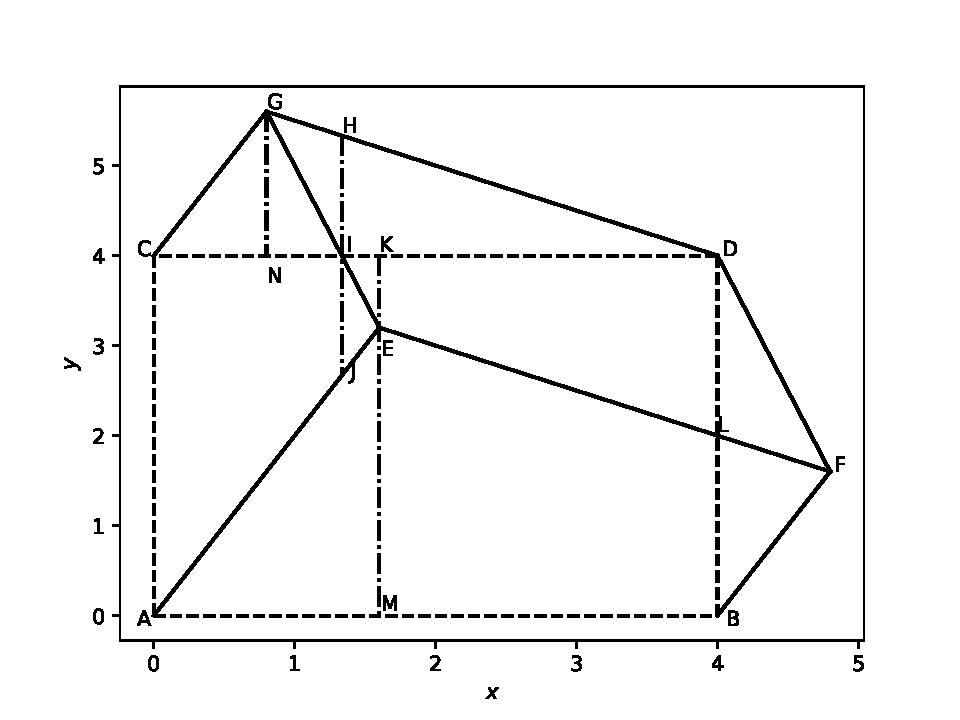
\includegraphics[width=\linewidth]{proj_xy.pdf}
  \caption{A boat.}
  \label{fig:boat1}
\end{figure}

\begin{table}
\begin{tabular}{|l l l l l l l l|}
\hline
Vertex&A&B&C&D&E&F&G\\
\hline
$x$&0&4&0&4&\sfrac{8}{5}&\sfrac{24}{5}&\sfrac{4}{5}\\
$y$&0&0&4&4&\sfrac{16}{5}&\sfrac{8}{5}&\sfrac{28}{5}\\
\hline
\hline
Vertex&H&I&J&K&L&M&N\\
\hline
$x$&\sfrac{4}{3}&\sfrac{4}{3}&\sfrac{4}{3}&\sfrac{8}{5}&4&\sfrac{8}{5}&\sfrac{4}{5}\\
$y$&\sfrac{16}{3}&4&\sfrac{8}{3}&4&2&0&4\\
\hline
\end{tabular}
\end{table}


\begin{table}
\caption{Double integrals.}
\begin{center}

\begin{tabular}{|l l l l l l l l|}
  $k$ & Vertices & $a$ & $b$  & $g_1$ & $g_2$ & $f_k$ & $\iint\limits_{\!R_k} f_k~dA$\\
  1 & AEM & 0 & \sfrac{8}{5}  & 0 & $2x$ &  $y$ & 2.7307 \\
  2 & MELB & \sfrac{8}{5} & 4  & 0 & -$\frac{1}{2}x+4$ & $y$ & 8.2560 \\
  3 & BLF & 4 & \sfrac{24}{5} & $2x-8$ & -$\frac{1}{2}x+4$ & $y-2(x-4)$ & 0.5333 \\
  4 & ACIJ & 0 & \sfrac{4}{3} & $2x$ & 4 & $2x$ & 3.9506\\
  5 & JIE & \sfrac{4}{3} & \sfrac{8}{5} & $2x$ & $-3x+8$ & $2x$ & 0.5058\\ 
  6 & EIK & \sfrac{4}{3} & \sfrac{8}{5} & $-3x+8$ & 4 &  $-x-y+8$ & 0.2939 \\ 
  7 & EKDL & \sfrac{8}{5} & 4 & $-\frac{1}{2}x+4$ & 4 &  $-x-y+8$ & 5.9520 \\ 
  8 & LDF & 4 & \sfrac{24}{5} & $-\frac{1}{2}x+4$ & $-3x+16$ & $-x-y+8-2(x-4)$ & 0.5333 \\ 
  9 & CGN & 0 & \sfrac{4}{5} & 4 & $2x+4$ & $2x-(y-4)$ & 0.3413 \\ 
  10 & NCI & \sfrac{4}{5} & \sfrac{4}{3} & 4 & $-3x+8$ & $2x-(y-4)$ & 0.6068 \\
  11 & ICH & \sfrac{4}{5} & \sfrac{4}{3} & $-3x+8$ & $-\frac{1}{2}x+6$ & $-x-y+8-(y-4)$&0.3160\\
  12 & IHD & \sfrac{4}{3}& 4  & 4 & $-\frac{1}{2}x+6$ & $-x-y+8-(y-4)$&1.5803\\
\end{tabular}
 
\end{center}

\end{table}

%$r_1(x) = \frac{1}{2}[\sqrt{17-4x^2}-1]$% ,
%$r_2(x) = \sqrt{-x^2-x+4}$, %$r_3(x) = \frac{1}{2}\sqrt{-x^2-(x-1)+4}$ en %$r_4(x) = \sqrt{-x^2-(x-1)+4}$.  


\begin{table}
\caption{Double integrals for sphere. $c_1 \approx 1.1861407$, $c_2 \approx 1.6861407$, $c_3 \approx 0.6861407$ and $c_4 \approx 1.3507811$. $r_1(x) = \frac{1}{2}[\sqrt{17-4x^2}-1]$,
$r_2(x) = \sqrt{-x^2-x+4}$, $r_3(x) = \frac{1}{2}\sqrt{-x^2-(x-1)+4}$ and $r_4(x) = \frac{1}{2}[\sqrt{21-4x^2}-1]$.} 
\begin{center}

\begin{tabular}{|l l l l l l l l|}
  $k$ & Vertices & $a$ & $b$  & $g_1$ & $g_2$ & $f_k$ & $\iint\limits_{\!R_k} f_k~dA$\\
  1 & ABD & 0 & 1& 0 & $x$ & $\sqrt{y}$ & ?\\
  2 & BLED& 1& $c_1$ & $x-1$ & $x$ & $\sqrt{y} - \sqrt{x-1}$& ?\\
  3 & LFE& $c_1$ & $c_2$ & $x-1$ & $r_1(x)$&$\sqrt{y} - \sqrt{x-1}$&?\\
  4 & ADC& 0 & 1 & $x$ & 1 & $\sqrt{x}$ & ?\\
  5 & CIG& 0 & $c_3$ & 1 & $x+1$ & $\sqrt{x}$ - $\sqrt{y-1}$ & ? \\
  6 & IDJG& $c_3$ & 1 & 1 & $r_2(x)$ & $\sqrt{x}$ - $\sqrt{y-1}$&?\\
  7 & DEJ& 1& $c_1$& $x$ & $r_2(x)$ & $\sqrt{x}$ - $\sqrt{y-1}$&? \\ 
  8 & EKG& $c_3$& $c_1$& $r_2(x)$ & $r_4(x)$ & $\sqrt{-x^2-y^2+4}-\sqrt{y-1}$&?\\ 
  9 & EHK& $c_1$& $c_4$& $x$& $r_4(x)$ & $\sqrt{-x^2-y^2+4}-\sqrt{y-1}$&?\\
  10& EMH& $c_1$& $c_4$& $r_1(x)$& $x$ & $\sqrt{-x^2-y^2+4}-\sqrt{x-1}$&?\\
  11& MFH& $c_4$& $c_2$& $r_3(x)$& $r_1(x)$ & $\sqrt{-x^2-y^2+4}-\sqrt{x-1}$&?\\ 
  %1 & AEM & 0 & \sfrac{8}{5}  & 0 & $2x$ &  $y$ & 2.7307 \\
  %2 & MELB & \sfrac{8}{5} & 4  & 0 & -$\frac{1}{2}x+4$ & $y$ & 8.2560 \\
  %3 & BLF & 4 & \sfrac{24}{5} & $2x-8$ & -$\frac{1}{2}x+4$ & $y-2(x-4)$ & 0.5333 \\
  %4 & ACIJ & 0 & \sfrac{4}{3} & $2x$ & 4 & $2x$ & 3.9506\\
  %5 & JIE & \sfrac{4}{3} & \sfrac{8}{5} & $2x$ & $-3x+8$ & $2x$ & 0.5058\\ 
  %6 & EIK & \sfrac{4}{3} & \sfrac{8}{5} & $-3x+8$ & 4 &  $-x-y+8$ & 0.2939 \\ 
  %7 & EKDL & \sfrac{8}{5} & 4 & $-\frac{1}{2}x+4$ & 4 &  $-x-y+8$ & 5.9520 \\ 
  %8 & LDF & 4 & \sfrac{24}{5} & $-\frac{1}{2}x+4$ & $-3x+16$ & $-x-y+8-2(x-4)$ & 0.5333 \\ 
  %9 & CGN & 0 & \sfrac{4}{5} & 4 & $2x+4$ & $2x-(y-4)$ & 0.3413 \\ 
  %10 & NCI & \sfrac{4}{5} & \sfrac{4}{3} & 4 & $-3x+8$ & $2x-(y-4)$ & 0.6068 \\
  %11 & ICH & \sfrac{4}{5} & \sfrac{4}{3} & $-3x+8$ & $-\frac{1}{2}x+6$ & $-x-y+8-(y-4)$&0.3160\\
  %12 & IHD & \sfrac{4}{3}& 4  & 4 & $-\frac{1}{2}x+6$ & $-x-y+8-(y-4)$&1.5803\\
\end{tabular}
 
\end{center}

\end{table}


 
\end{section}



\end{document}
 